%++++++++++++++++++++++++++++++++++++++++
% Don't modify this section unless you know what you're doing!
\documentclass[letterpaper,11pt]{article}
\usepackage{tabularx} % extra features for tabular environment
\usepackage{amsmath}  % improve math presentation
\usepackage{graphicx} % takes care of graphic including machinery
\usepackage[margin=1.3in,letterpaper]{geometry} % decreases margins
\usepackage{cite} % takes care of citations
\usepackage[final]{hyperref} % adds hyper links inside the generated pdf file
\usepackage{titlesec}
\usepackage{verbatim}
\usepackage{ragged2e}
\usepackage{amssymb}
\usepackage{tikz}
\usetikzlibrary{calc}
\tikzset{axis line style/.style={thin, gray, -stealth}}
\newcommand*{\TickSize}{2pt}
\setcounter{secnumdepth}{3}
\newtheorem{theorem}{Theorem}[section]
\newtheorem{property}{Property}[theorem]
\newtheorem{lemma}{Lemma}[theorem]

\makeatletter
\def\BState{\State\hskip-\ALG@thistlm}
\makeatother
\hypersetup{
	colorlinks=true,       % false: boxed links; true: colored links
	linkcolor=blue,        % color of internal links
	citecolor=blue,        % color of links to bibliography
	filecolor=magenta,     % color of file links
	urlcolor=blue
}
\newcommand\given[1][]{\:#1\vert\:}
\usepackage{listings}
\usepackage{array}
\usepackage{diagbox}
\usepackage{multicol}
\lstset{
  basicstyle=\ttfamily,
  mathescape
}
\usepackage{caption}
\usepackage{hyperref}

\usepackage{fvextra} % loads also fancyvrb
\usepackage{xpatch}

\DeclareMathVersion{ttmath}
\DeclareSymbolFont{latinletters}{OT1}{\ttdefault}{m}{n}
%\SetSymbolFont{latinletters}{ttmath}{OT1}{\ttdefault}{m}{n}
\SetSymbolFont{letters}{ttmath}{OML}{ccm}{m}{it}
\SetSymbolFont{symbols}{ttmath}{OMS}{ccsy}{m}{n}
\SetSymbolFont{largesymbols}{ttmath}{OMX}{ccex}{m}{n}

\newcommand{\changeletters}{%
  \count255=`A
  \advance\count255 -1
  \loop\ifnum\count255<`Z
    \advance\count255 1
    \mathcode\count255=\numexpr\number\symlatinletters*256+\count255\relax
  \repeat
  \count255=`a
  \advance\count255 -1
  \loop\ifnum\count255<`z
    \advance\count255 1
    \mathcode\count255=\numexpr\number\symlatinletters*256+\count255\relax
  \repeat
  \count255=`0
  \advance\count255 -1
  \loop\ifnum\count255<`9
    \advance\count255 1
    \mathcode\count255=\numexpr\number\symlatinletters*256+\count255\relax
  \repeat
}

\xapptocmd{\ttfamily}{\mathversion{ttmath}\changeletters}{}{}
%++++++++++++++++++++++++++++++++++++++++


\begin{document}

\title{\textbf{Practical Network Defense}\\ \bigskip \large Third Assignment - University ``La Sapienza"}
\date{2020-13-06}
\author{\textbf{Group 27}: Nicola Bartoloni 1909908 - Valerio Trenta 1856471}
\maketitle

\section{Scope and Initial Considerations}
The scope of this assignment is to setup a \textbf{Virtual Private Network} through \textbf{OpenVPN} in \textbf{OPNSense} to allow three authenticated \textit{Road Warriors} to access the internal subnetworks of \textbf{ACME Co.}, and to grant the usage of a \textbf{proxy server} on machine located at \textbf{100.100.6.3} -  which corresponds to domain \textbf{proxy.acme.group27} to the very same authenticated internal clients of the network to reach the \textbf{WAN} outside the \textbf{Main Firewall}.\\
Since these tasks are going to allow connections from the outside - even if authenticated and thus probably secured - it is a good idea to make sure, as a first step, that every user on each of the internal machines is protected by a strong password, and we will probably also have to confirm that the SSH protocol on each machine behaves as we expect it to behave - some of the \textit{root} accounts are already disabled by SSH on some machines, but some are still accepting connections based on basic authentication.\\
The next paragraphs will only deal with the two services we want to setup in the target network - \textbf{VPN} and \textbf{proxy server}.

\newpage
\section{VPN Setup}
We can define the \textbf{road warriors}, in our case, as a set of three users - \textit{Becca, Huck and Jim} - which we want to be able to authenticate and then connect to the internal subnetworks in the \textbf{ACME Co.} target network from the \textbf{WAN} interface on the \textbf{Main router} via a \textbf{Virtual Private Network}.\\
To this end, in order to setup a \textbf{VPN} on the \textbf{Main router}, we exploit the \textbf{OPNSense} administration panel and then navigate to \textbf{VPN $->$ OpenVPN $->$ Servers}, where we can \textbf{add a new server} to which the \textbf{road warriors} will refer to authenticate and configure their \textbf{VPN}. \textbf{Figure 1, 2, 3} show the server we created and all the parameters - protocol, port, cryptographic and tunnel settings - that we chose to adopt.\\
\begin{figure}[!htb]
\centering
\begin{minipage}{.33\textwidth}
  \centering
  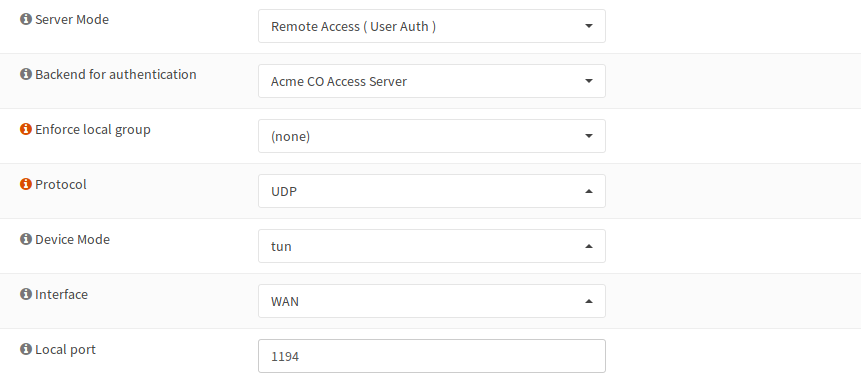
\includegraphics[width=1\textwidth]{vpnserver1.png}
  \caption[a]{VPN Server's general settings with protocol and port.}\label{fig:1}
\end{minipage}%
\begin{minipage}{.33\textwidth}
  \centering
  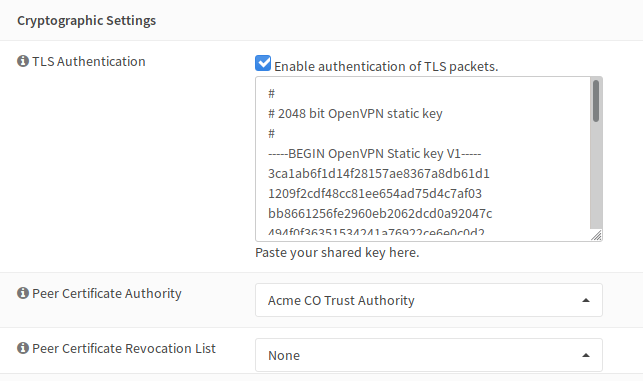
\includegraphics[width=1\textwidth]{vpnserver2.png}
  \caption[a]{VPN Server's crypto settings (1).}\label{fig:2}
\end{minipage}
\begin{minipage}{.33\textwidth}
  \centering
  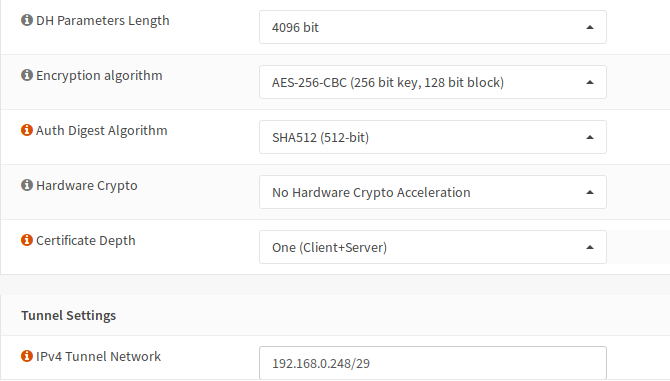
\includegraphics[width=1\textwidth]{vpnserver3.png}
  \caption[a]{VPN Server's crypto settings (2) and IP tunneling address.}\label{fig:3}
\end{minipage}
\end{figure}

Also, under \textbf{System $->$ Servers} we setup a new \textit{Acme CO Access Server} which will be exploited to actually access the \textbf{VPN Server}, exploiting an access strategy based on a \textit{Local Database $+$ Timebased One Time Password}, with the  \textbf{OTP} being provided by \textit{Google Authenticator} and thus having length 6. Before actually implementing the \textbf{VPN}, it is also necessary to define the authentication system and how the three users will be able to actually access, but this is discussed in the fourth paragraph.\\
In order to grant the \textbf{road warriors} to only access through \textbf{SSH} protocol the \textit{internal machines} - i.e., machines on \textit{Internal Servers} and \textit{Clients} subnetworks - the rules at the \textbf{Main firewall} had to be changed as follows:\\
\begin{itemize}
\item at \textbf{WAN} interface, a \textbf{Pass} rule was added to accept every connection from any source on destination port \textbf{1194} for procotol \textbf{UDP}, so to enable connections with \textbf{OpenVPN Server};
\item a new interface, \textbf{OpenVPN}, was automatically generated by \textbf{OPNSense} once the \textbf{OpenVPN Server} was created: here, the firewall allows only connections with source IP address \textit{192.168.0.248$/$29} (being the one specified in the \textbf{IP Tunneling} field of our server) to perform the users' authentication, and then connections with same source IP address and destination IP address being either in the \textit{Internal Servers} or in the \textit{Clients} subnetworks on destination port 22.
\end{itemize}

Similar rules had also to be added on the interfaces of the \textbf{Internal router} to allow hosts in the two target subnetworks to accept connections with the \textbf{VPN}.

\section{Proxy Setup}
We want to setup a \textbf{proxy service} at \textbf{proxy.acme.group27} that can be exploited only by \textit{authenticated} users located in the \textit{Clients} subnetwork. For the sake of simplicity, the users we will accept and authenticate are the same we have defined previously for the \textbf{road warriors} set.\\
The setup is carried out entirely in the \textbf{proxy.acme.group27} machine, and even if this machine gives us the chance to setup an \textit{HTTP Squid Proxy service} through \textbf{zentyal} administration panel, we decide to setup \textbf{Squid} directly via the \textit{squid.conf} file as pictured in \textbf{Figure 4} (next page).\\
We decide to implement a \textbf{non-transparent proxy} given the requirements for the service, so that the users in the \textit{Clients} subnet will have to manually configure their browsers.\\
The service can be accessed, as anticipated in the previous assignment, on port \textbf{3128} via \textbf{HTTP}. Apart from defining several default \textbf{acl}s for different safe ports, we define an \textbf{acl} named \textbf{Clients$\_$net} to identify the target \textit{Clients} subnetwork, and an \textbf{acl} named \textbf{authenticated} which identifies users that have been successfully \textbf{authenticated} through module \textbf{basic$\_$ncsa$\_$auth} (\textbf{Figure 5}).\\
Notice that every user-password pair is stored under the file \textit{$/$etc$/$squid$/$passwd}, this and the whole authentication procedure will be discussed on the next paragraph.\\
At this point, with line \textit{http$\_$access allow Clients$\_$net authenticated} we grant access to users that are in the desired internal subnet and that have been successfully authenticated. Every other connection is denied through default line \textit{http$\_$access deny all}, and reply access is allowed if not denied before as default.\\
As pictured in the detail on \textbf{Figure 6}, as requested by the assignment the \textbf{proxy service} holds a \textbf{cache} and \textbf{log file} for it, as well as an \textbf{access.log} file to log all the accesses and operations performed by the authenticated users.\\
The firewall rules were already setup so that this service could be available from the \textit{Clients} subnetwork and so that its machine had Internet access. So, in order to visit one of white-listed websites - \textbf{cybersecurity.uniroma1.it} which has IP address \textbf{151.100.17.12} - we only need to start the daemon of the \textbf{Squid} service via command \textit{systemctl start squid} after having it enabled, and then setup the \textit{Firefox Browser} on the Kali machine so that it knows how to contact the service: \textit{Firefox $->$ Preferences $->$ Network Settings $->$ Settings $->$ Manual proxy configuration} with the very well known values (100.100.6.3 and 3128 as port) to be exploited with all protocols.\\
Results are showed in the sixth paragraph.\\

\begin{figure}[!htb]
\centering
\begin{minipage}{.33\textwidth}
  \centering
  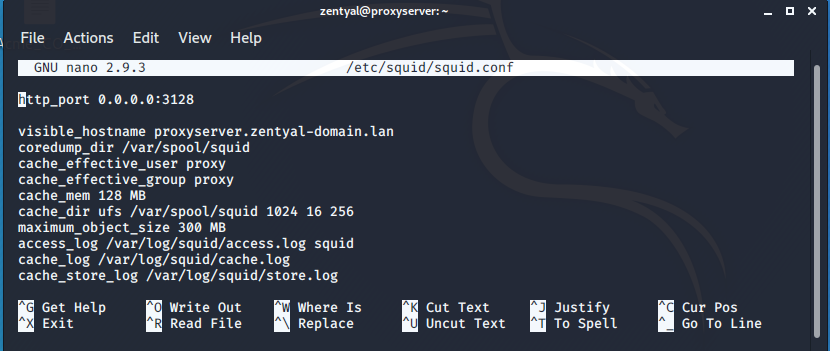
\includegraphics[width=1\textwidth]{squidConf1.png}
  \caption[a]{Beginning of the squid.conf file with the 3128 port specified.}\label{fig:4}
\end{minipage}%
\begin{minipage}{.33\textwidth}
  \centering
  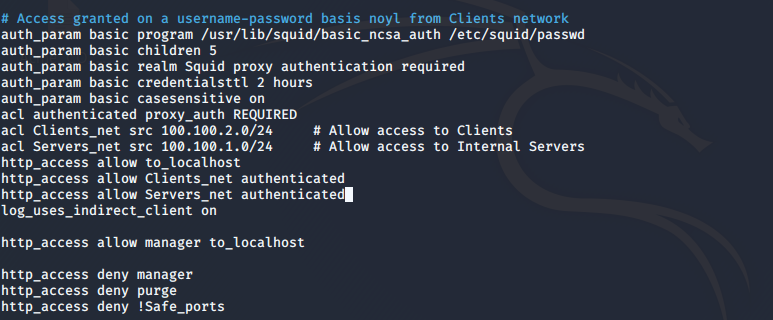
\includegraphics[width=1\textwidth]{squidConf2.png}
  \caption[a]{acls defined to restrict the access to the service.}\label{fig:5}
\end{minipage}
\begin{minipage}{.33\textwidth}
  \centering
  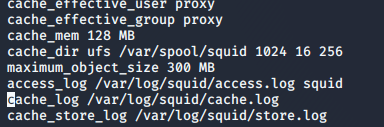
\includegraphics[width=1\textwidth]{squidConf3.png}
  \caption[a]{Configuring log files for cache and accesses to the service.}\label{fig:6}
\end{minipage}
\end{figure}

\newpage
\section{Authentication}
Both services we implemented in this assignment require a \textit{basic authentication} in order to be accessed. Users to be authenticated are the three we already mentioned in the previous paragraphs, belonging to the \textbf{road warriors} set: \textit{Becca, Huck and Jim}. Each of them has two unique passwords, different from each other, one for the \textbf{VPN service} and one for the \textbf{Proxy service}.\\

\subsection{VPN Authentication}
Access rules for the \textbf{VPN service} have been defined on the \textbf{OPNSense} administration panel located at the \textbf{Main router}, under the \textbf{System} tab. The three users have been assigned to the \textbf{ROADWARRIORS} group and, for each of them, an \textbf{RSA Public Key} has been created and assigned for \textbf{TLS Authentication} process of \textbf{OpenVPN}. Moreover, each of the three users holds a unique password and a \textbf{One Time Password} - a six-characters token provided by \textbf{Google Authenticator}.\\
This way, in order for one of the users to authenticate to the \textbf{OpenVPN service}, it must necessarily own \textit{three requirements}:\\
\begin{itemize}
\item its own unique \textbf{.ovpn client exported file} located under the tab \textbf{OpenVPN $->$ Clien Export}, which must be exploited by the client machine's \textbf{openvpn} tool to retrieve the server's location, port, parameters and perform the \textbf{TLS Authentication};
\item its own unique and static \textbf{password} defined under its own profile on the \textbf{OPNSense} administration panel;
\item its own \textbf{OTP} provided by \textbf{Google Authenticator}
\end{itemize}

when these three requirements are met, the user can easily access to the \textbf{OpenVPN} service and reach the internal machines as desired.

\subsection{Proxy Authentication}
As already mentioned, the \textbf{Proxy Service} is only reachable when the client's IP address is found to belong to the \textbf{Clients subnetwork} (\textit{100.100.2.0$/$24}).\\
Moreover, we perform once again \textbf{basic authentication} so that only internal clients owning a \textit{username-password} pair that is known to the service can actually authenticate and exploit it. Once again, the three authorized users to authenticate to the service are \textit{Becca, Huck and Jim}. Each of them holds a unique password, different from the ones we defined for the \textbf{OpenVPN service}, whose \textit{hash} has been stored through the \textbf{htpasswd} tool under the file \textit{$/$etc$/$squid$/$passwd} located at \textbf{proxy.acme.group27}, so that the passwords are not stored in clear.\\
This way, each time an user from the \textit{internal Clients subnetwork} accesses a web browser having the \textbf{Proxy service} set, a dialog pops up requesting username and password to authenticate: if the authentication fails, the service won't be reached and the user will not be able to exploit it and thus surf the Internet.\\
Details about the basic authentication exploited in the \textbf{Squid} service were also given in the previous paragraph: passwords are \textit{case sensitive} and the service only remembers an authenticated user for \textit{2 hours} if he doesn't disconnect from the service itself. After 2 hours, the service will require the user once again to provide their credentials.

\newpage
\section{Tests}
Tests that we run on both the two services aimed at verifying their correct behavior - i.e., that the two services were actually confgiured correctly so to be exploited as desired by non-malicious users - and that their setup does not hold a negative impact on the policy implemented in the previous assignment - i.e., the services can be only exploited by authenticated users under certain already mentioned conditions.

\subsection{Testing the VPN}
The \textbf{OpenVPN} service implemented on the \textbf{Main firewall} must be exploited only by an \textit{authenticated user} - that is, a user who owns \textit{three distinct credentials} in order to prove its identity and correctly gain access to the service. These three credentials are: the \textbf{.ovpn} file provided by the \textbf{OPNSense} portal correctly specifying the \textbf{valid cryptographic parameters} to authenticate the user on the \textbf{OpenVPN server}. This file holds the parameters that we previously showed, like port number, authentication type and the cryptographic functions to be arranged during the handshake between client and server, as pictured in \textbf{figure 7}.

\begin{figure}[!htb]
\centering
\begin{minipage}{.33\textwidth}
  \centering
  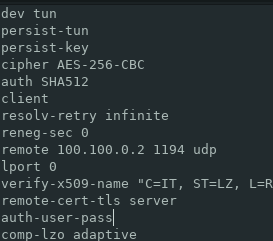
\includegraphics[width=1\textwidth]{ovpnParams.png}
  \caption[a]{Parameters in the .ovpn client file.}\label{fig:7}
\end{minipage}%
\end{figure}

Along with these parameters, the file also holds two different \textbf{keys}, one being the \textbf{certificate} for client to server authentication, the other being the \textbf{2048 bit OpenVPN static key} provided during the \textbf{TLS authentication}.\\
The other two credentials are the pair \textbf{(username, password)} specified under the settings of the \textbf{OPNSense} pannel - e.g., \textbf{Becca} as username and \textbf{password} as her password - and, furthermore, a \textbf{six characters token} provided by the \textbf{Google Authenticator}, which is a \textbf{One Time Password} different for each of the three users to be provided along the user's own static password during the basic authentication phase.\\
Once the \textbf{OpenVPN} terminates the intialization and the user authenticates successfully, he can exploit the new \textbf{tunnel} to gain access to the machines under the \textbf{Clients subnetwork} as requested by the assignment, through the \textbf{SSH} protocol on its own machine located in the \textbf{WAN} - once the \textbf{SSH} service has been enabled on the client's machines and routing has been appropriately configured on the local machine. This is the only operation that the \textbf{road warriors} are enabled to perform - they do not have access to the other subnetworks in the whole network, but we should stress the point that, once they gain access to one of the machines in the \textbf{Clients subnetwork}, they do have access to any other machine in the internal and DMZ subnet, which should actually be a desired feature.\\
\textbf{Figure 8} pictures the successful remote access of user \textbf{Becca} to the \textbf{kali machine} via the \textbf{OpenVPN service}. As far as we know, the only vulnerability that is introduced in the network with this service, is that now the \textbf{Main firewall} accepts connections on port \textbf{1194} on the \textbf{WAN} interface, and that the machines in the \textbf{Clients subnetwork} now accept connections with protocol \textbf{SSH} on \textbf{port 22} if and only if the request is coming from the \textbf{OpenVPN} tunnel - that is, only authenticated users should be actually able to login via \textbf{SSH} on those machines from the \textbf{WAN}.\\

\begin{figure}[!htb]
\centering
\begin{minipage}{.80\textwidth}
  \centering
  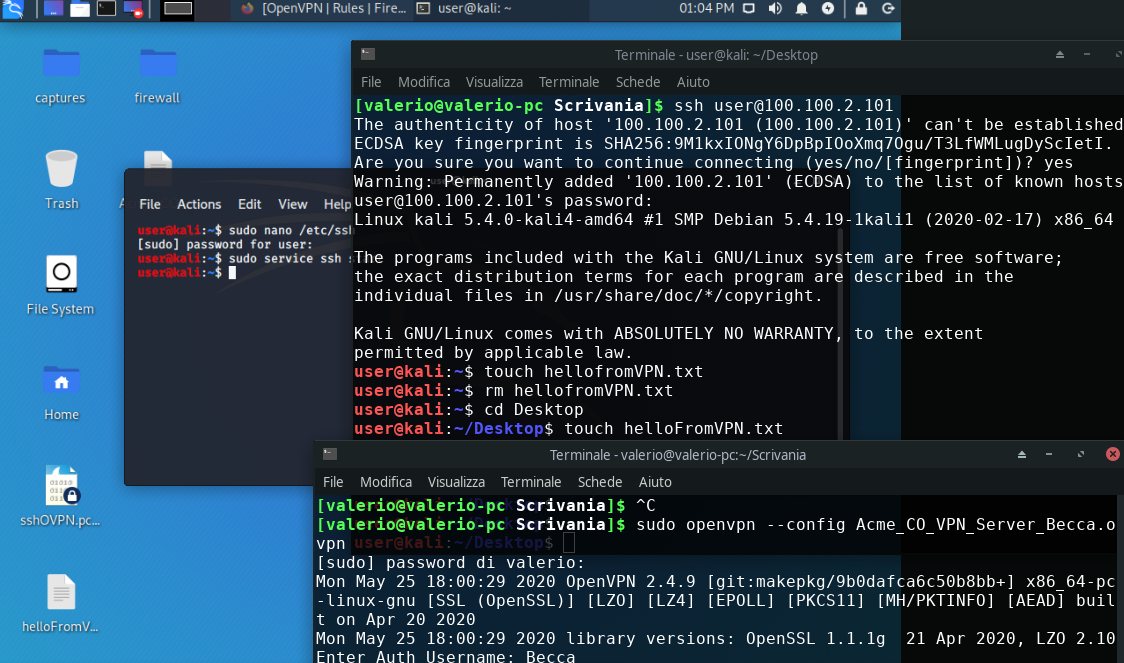
\includegraphics[width=1\textwidth]{OVPNaccessViaSSH.png}
  \caption[a]{User Becca accessing the Kali Machine via OpenVPN-SSH.}\label{fig:8}
\end{minipage}%
\end{figure}

\subsection{Testing the Proxy service}
We want the \textbf{squid proxy service} on the \textbf{proxy machine} to accept only users that have authenticated and are located in the \textbf{Clients subnetwork}, thus connections coming from a different subnetwork or the \textbf{WAN} are rejected a priori. In the \textbf{Kali machine}, we setup \textbf{Firefox browser} preferences so that it connects to the \textbf{proxy machine} requesting the \textbf{squid} service on port \textbf{3128} for every HTTP or HTTPS connection but those that have destination in the \textbf{Internal}, \textbf{External services} or \textbf{DMZ} subnetworks - \textit{manual configuration}. The figures below picture the desired behavior of both the services and the client's browser, which is now able to \textit{go out} in the \textbf{WAN} once the user is authenticated.\\

\begin{figure}[!htb]
\centering
\begin{minipage}{.5\textwidth}
  \centering
  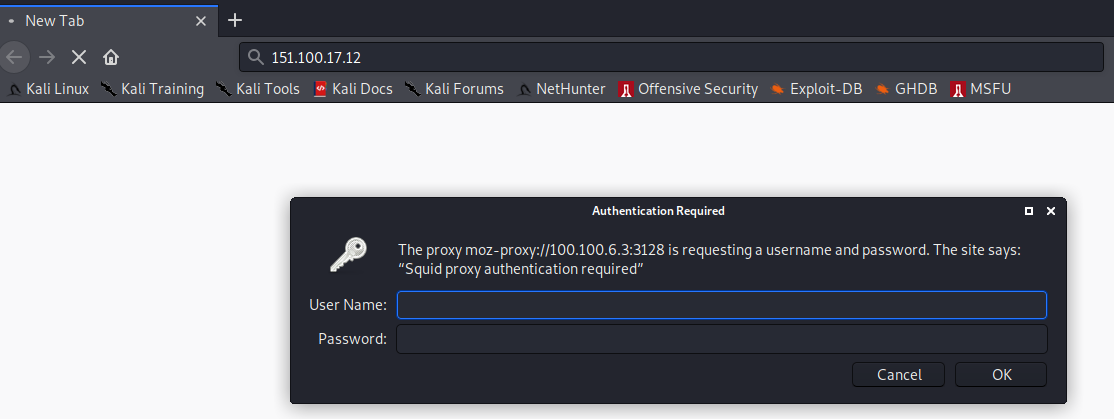
\includegraphics[width=1\textwidth]{proxyAuth.png}
  \caption[a]{Authentication procedure in the Kali machine's browser.}\label{fig:9}
\end{minipage}%
\begin{minipage}{.5\textwidth}
  \centering
  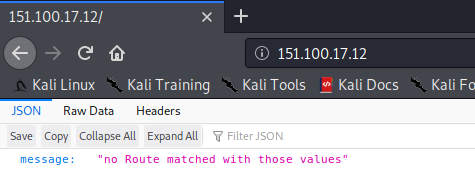
\includegraphics[width=1\textwidth]{proxyAuthed.png}
  \caption[a]{Successfully authenticated user can exploit proxy to display web pages outside of the network.}\label{fig:10}
\end{minipage}%
\end{figure}

\newpage
\section{Final remarks}
The testing phase showed us that the policy, if correctly interpreted, was implemented as specified by the assignment.\\
Some extra measures could have been taken, and they are very similar to the ones we have seen in the first assignment: we need to perform Linux hardening via sudo and hardening of the SSH protocol for all the machines in the DMZ and Internal Service subnetworks, and we need to change the default passwords for services such as \textbf{Zentyal} too and for users on the machines as well.\\
We should also stress the fact that, even if we found out that some of the machines had the SSH login via their \textit{root} account disabled by default, the scope of this assignment was to focus mainly on the \textbf{firewall rules} to be defined to achieve our goals and implement the given policy: this means that link$-$layer attacks were not taken into consideration, and this may be a critical vulnerability in our network. indeed, notice that every machine can be accessed through SSH or other protocols by any other machine on its same subnetwork - i.e., \textit{dc} can access \textit{logserver} through any protocol. This is because the rules we defined to implement our policy are placed on the two firewall$-$routers, which obviously do not handle packets exchanged between hosts in the same subnetwork: to overcome this issue, probably some extra rules should also be defined locally on each machine via \textit{iptables} - but this was out of our scope for this assignment.\\
We should also mention the fact that the \textbf{UDP} protocol was chosen to implement the \textbf{rsyslog} service, which could be also implemented through \textbf{TCP} protocol - commonly considered more secure - and maybe forced to exploit secure channels. Again, our goal here was to enable the service and enforce the policy via firewall rules, but we should stress the fact that just by exploiting TCP, this service may be hardened.\\
Also, as a last step, when the whole configuration going on in these assignments is over, we should at least enable only one machine in the \textbf{Clients} subnetwork - the \textbf{Kali} machine, probably - to connect via HTTP service to the two routers, for administration and practical reasons, so as we mentioned in the previous paragraphs, the rule enabling these connections should be actually disabled as a last step.

\newpage

\end{document}
